\documentclass[areasetadvanced]{scrartcl}

\usepackage[utf8]{inputenc}
\usepackage[T2A]{fontenc}
\usepackage[english,russian]{babel}

\usepackage[footskip=1cm,left=25mm, right=15mm, top=20mm, bottom=20mm]{geometry}
\usepackage{setspace}
\usepackage{amsmath, amssymb}  % Объединено в одну строку
\usepackage{graphicx}
\usepackage{booktabs,longtable}
\usepackage{tikz}
\usetikzlibrary{arrows.meta}
\usepackage{float}
\usepackage{dashrule}
\usepackage{fancyhdr} % оформление отчёта
\usepackage{hyperref} % оформление отчёта
\usepackage{parskip}
\usepackage[strings]{underscore}

\usepackage{textcomp, enumitem}
\usepackage{indentfirst}
\usepackage{graphicx}
\usepackage{algorithm}
\usepackage{algpseudocode}
\usepackage{array}  % Для использования команды m{}
\usepackage{geometry}
\usepackage{afterpage}
\usepackage{minted}
\setcounter{secnumdepth}{3}  % Включает нумерацию для subsubsection
\setcounter{tocdepth}{3}     % Включает subsubsection в содержание
\usepackage{listings} % Если используете listings

\tikzstyle{block} = [rectangle, rounded corners, minimum width=3cm, minimum height=1cm, text centered, draw=black, fill=lightgray]

\setkomafont{sectioning}{\normalfont\bfseries} % для заголовков разделов и подразделов
\setkomafont{section}{\normalfont\Large\bfseries}
\setkomafont{subsection}{\normalfont\large\bfseries}
\setkomafont{subsubsection}{\normalfont\large\bfseries}
\setkomafont{paragraph}{\normalfont\large\bfseries} % для заголовков параграфов (если они есть)

\lstset{
  language=R,
  basicstyle=\ttfamily\small,
  keywordstyle=\color{blue}\bfseries,
  stringstyle=\color{red},
  commentstyle=\color{green!70!black},
  numbers=left,
  numberstyle=\tiny,
  stepnumber=1,
  numbersep=10pt,
  showstringspaces=false,
  breaklines=true,
  frame=single
}

\setcounter{tocdepth}{2}
\begin{document}
\sloppy
	\thispagestyle{empty}
	\begin{center}
		\large{МИНОБРНАУКИ РОССИИ} \par
		\vspace{0.3cm}
		\normalsize
		{ФЕДЕРАЛЬНОЕ ГОСУДАРСТВЕННОЕ АВТОНОМНОЕ ОБРАЗОВАТЕЛЬНОЕ УЧРЕЖДЕНИЕ ВЫСШЕГО ОБРАЗОВАНИЯ} \par
		\vspace{0.3cm}
		\textbf{\guillemotleft САНКТ-ПЕТЕРБУРГСКИЙ ПОЛИТЕХНИЧЕСКИЙ}
		\textbf{УНИВЕРСИТЕТ ПЕТРА ВЕЛИКОГО\guillemotright} \par
		\vspace{0.3cm}
		{Институт компьютерных наук и кибербезопасности}\par
		{Высшая школа технологий искусственного интеллекта}\par
	\end{center}
	\vfill
	\begin{center}
		{\large Отчёт по дисциплине \guillemotleft Математическая статистика\guillemotright}\par
		{\huge   ИДЗ №3
		
		\guillemotleft Классическая статистика\guillemotright}\par
            {\huge Вариант \textbf{№25}}
         
	\end{center}
	\vfill
	\begin{flushleft}
		Студент: \hspace{1.8cm} \rule[0pt]{2.5cm}{0.5pt}\hfill Салимли Айзек Мухтар Оглы\par
		\vspace{1.5cm}
		Преподаватель: \hspace{0.55cm} \rule[0pt]{2.5cm}{0.5pt}\hfill  Малов Сергей Васильевич
	\end{flushleft}
	\vspace{0.5cm}
	\begin{flushright}
		\guillemotleft \rule[0pt]{0.8cm}{0.5pt}\guillemotright \rule[0pt]{2cm}{0.5pt} 20\rule[0pt]{0.5cm}{0.5pt} г.
	\end{flushright}
	\vfill
	\begin{center}
		Санкт-Петербург, 2025
	\end{center}
	\newpage
	\tableofcontents
	\newpage
\section*{Введение}
	\addcontentsline{toc}{section}{Введение}
В данном отчете, приведено решение и реализация двух задач под вариантом №25, из ИДЗ№3. Для реализации программной части решения использоавлись:
\begin{itemize}
    \item Среда разработки: Visual Studio Code
    \item Язык программирования: R 4.
\end{itemize}
\newpage
\section{Постановка задачи}

\textbf{№1:
В результате эксперимента получены данные, приведенные в таблице 1.}
\begin{enumerate}
    \item Построить вариационный ряд, эмпирическую функцию распределения и гистограмму частот.

    \item  Вычислить выборочные аналоги следующих числовых характеристик:
    \item (і) математического ожидания, (іi) дисперсии, (ііi) медианы, (iv) асимметрии, (v) эксцесса,(vi) вероятности $P(X \in [a, b])$.

    \item В предположении, что исходные наблюдения являются выборкой из распределения Пуассона, построить оценку максимального правдоподобия параметра $\lambda$, а также оценку $\lambda$ по методу моментов. Найти смещение оценок.

    \item Построить асимптотический доверительный интервал уровня значимости $\alpha_1$ для параметра $\lambda$ на базе оценки максимального правдоподобия.
    \item Используя гистограмму частот, построить критерий значимости $\chi^2$ проверки простой гипотезы согласия с распределением Пуассона с параметром $\lambda_0$. Проверить гипотезу на уровне значимости $\alpha_1$. Вычислить наибольшее значение уровня значимости, на котором еще нет оснований отвергнуть данную гипотезу.

    \item Построить критерий значимости $\chi^2$ проверки сложной гипотезы согласия с распределением Пуассона. Проверить гипотезу на уровне значимости $\alpha_1$. Вычислить наибольшее значение уровня значимости, на котором еще нет оснований отвергнуть данную гипотезу.

    \item Построить наиболее мощный критерий проверки простой гипотезы пуассоновости с параметром $\lambda = \lambda_0$ при альтернативе пуассоновости с параметром $\lambda = \lambda_1$. Проверить гипотезу на уровне значимости $\alpha_1$. Что получится, если поменять местами основную и альтернативную гипотезы?

    \item В пунктах (3)-(6) заменить семейство распределений Пуассона на семейство геометрических распределений
\end{enumerate}

\[\textbf{P}_\lambda(X = k) = \frac{\lambda^k}{(\lambda+1)^{k+1}}, k = 0,1,\dots\]

\textbf{Таб.1: } $\alpha_1 = 0.002, a = 0.00, b = 1.79, \lambda_0 = 0.60, \lambda_1 = 1.40$\\
\{ 0 0 2 1 0 0 0 0 0 1 0 1 0 0 0 2 0 2 1 0 1 1 0 1 1 3 0 0 0 0 0 1 0 0 0 0 4 1 5 2 0 0 2 0 0 1 1 0 0 1\}

\textbf{№2:
В результате эксперимента получены данные, приведенные в таблице 2.}
\begin{enumerate}
	\item Построить вариационный ряд, эмпирическую функцию распределения, гистограмму и полигон частот с шагом $h$.
	\item Вычислить выборочные аналоги следующих числовых характеристик:
	(і) математического ожидания, (іі) дисперсии, (іі) медианы, (iv) асимметрии, (v) эксцесса,
	(vi) вероятности $\textbf{P}(X \in [c,d])$
	\item В предположении, что исходные наблюдения являются выборкой из показательного распределения, построить оценку максимального правдоподобия параметра $\lambda$ и соответствующую оценку по методу моментов. Найти смещение оценок.
	\item Построить асимптотический доверительный интервал уровня значимости $\alpha_2$ для параметра $\lambda$ на базе оценки максимального правдоподобия.
	\item С использованием теоремы Колмогорова построить критерий значимости проверки простой гипотезы согласия с показательным распределением с параметром $\lambda_0$. Проверить гипотезу на уровне значимости $\alpha_2$. Вычислить наибольшее значение уровня значимости, на котором нет оснований отвергнуть данную гипотезу.
	\item Используя гистограмму частот, построить критерий значимости $\chi^2$ проверки простой гипотезы согласия с показательным распределением с параметром $\lambda_0$. Проверить гипотезу на уровне $\alpha_2$. Вычислить наибольшее значение уровня значимости, на котором еще нет оснований отвергнуть данную гипотезу.
	\item Построить критерий проверки значимости $\chi^2$ сложной гипотезы согласия с показательным распределением.
	Проверить гипотезу на уровне $\alpha_2$. Вычислить наибольшее значение уровня значимости, на котором еще нет оснований отвергнуть данную гипотезу.
	\item Построить наиболее мощный критерий проверки простой гипотезы о показательности с параметром $\lambda = \lambda_0$ при альтернативе показательности с параметром $\lambda = \lambda_1$. Проверить гипотезу на уровне значимости $\alpha_2$. Что получится, если поменять местами основную и альтернативную гипотезы?
	\item В пунктах (3)-(8) заменить семейство показательных распределений на семейство гамма-распределений с плотностями $f(x) = \frac{\sqrt\lambda  e^{-\lambda x/2}}{\sqrt{2\pi x}}$ (использовать таблицу распределений $\chi_1^2$)
\end{enumerate}
\textbf{Таб.2: } $\alpha_2 = 0.001, c = 2.40, d = 6.00,h = 1.20, \lambda_0 = 0.20, \lambda_1 = 0.33$\\
\{10.34 2.18 8.80 2.28 1.95 0.85 3.73 10.26 5.01 0.70 2.38 0.25 0.45 0.31 1.73 2.67 1.00 1.59 14.28 2.14 1.85 0.67 2.70 2.07 5.31 6.37 3.24 3.27 1.31 2.75 6.06 1.05 0.86 2.43 0.03 3.70 0.11 1.06 6.28 0.55 9.07 6.52 0.94 2.61 0.89 1.67 0.24 1.68 3.34 1.38 \}

\newpage
%=================================================================
%                     З А Д А Ч А   №1
%=================================================================
\section{Математическое описание. Задача №1}
\subsection{Вариационный ряд, ЭФР, гистограмма}
\begin{itemize}
  \item Вариационный ряд:
        \(0^{(29)},\,1^{(13)},\,2^{(5)},\,3,4,5\) (\(n=50\)).
  \item Эмпирическая функция распределения
        \(\widehat F_n(x)=\dfrac1n\sum_{i=1}^{n}\mathbf 1_{\{X_i\le x\}}\).
  \item См. рис.~\ref{fig:ecdf1}–\ref{fig:hist1}.
\end{itemize}

\subsection{Выборочные характеристики}
\[
\bar X=0.7000,\quad
s^{2}=1.1939,\quad
\tilde X=0,\quad
\gamma_1=2.1022,\quad
\gamma_2=8.3810,\quad
\mathbf P\!\bigl\{0\le X\le1.79\bigr\}=0.84.
\]


\subsection{Подробные оценки параметра \(\lambda\)}
\paragraph{Оценка максимального правдоподобия.}
Пусть \(X_i\sim\mathrm{Pois}(\lambda)\). Лог-правдоподобие
\[
\ell(\lambda)=\sum_{i=1}^{n}\!\Bigl(x_i\ln\lambda-\lambda-\ln x_i!\Bigr)
             =(\Sigma x)\ln\lambda-n\lambda+\text{const}.
\]
\[
\frac{\partial\ell}{\partial\lambda}=0
\;\Longrightarrow\;
\hat\lambda_{\text{MLE}}=\frac{\Sigma x}{n}=0.7000.
\]

\textbf{Ответ:}
для распределения Пуассона \(\mathbb E[X]=\lambda\), поэтому
\(\operatorname{Bias}(\hat\lambda)=\mathbb E[\bar X]-\lambda=0\).

Фишерова информация \(I(\lambda)=\dfrac{n}{\lambda}\),
\(\operatorname{Var}\hat\lambda_{\text{MLE}}=\dfrac{\lambda}{n}=0.014\).

\paragraph{Оценка методом моментов.}
Для распределения Пуассона
\(\mathbb E[X]=\lambda\). Приравниваем к \(\bar X\):
\(\hat\lambda_{\text{ММ}}=\bar X=0.7000\) (совпадает с MLE).

\paragraph{Нормальное приближение для \(\hat\lambda\).}
\[
\hat\lambda\sim\mathcal N\!\Bigl(\lambda,\;\tfrac{\lambda}{n}\Bigr)
\quad\Rightarrow\quad
Z=\frac{\hat\lambda-\lambda}{\sqrt{\lambda/n}}\xrightarrow{d}\mathcal N(0,1).
\]

\subsection{Асимптотический доверительный интервал (\(\alpha_1=0.002\))}
\[
z_{0.999}=3.0902,\quad
CI_{99.8\%}= \hat\lambda\pm
3.0902\,\sqrt{\frac{\hat\lambda}{n}}
           =0.7000\pm0.3656=[0.3344;1.0656].
\]
\newpage
\subsection{Критерий \(\chi^{2}\). Простая гипотеза}
\begin{longtable}{ccccccc}
\caption{Группы при $H_0:\lambda_0=0.6$}\label{tab:chi1}\\[-1pt]\toprule
$i$ & класс & $n_i$ & $p_i$ & $E_i=np_i$ & $r_i$ & $r_i^2$\\\midrule
1 & $k=0$ & 29 & 0.5488 & 27.441 & 0.298 & 0.089\\
2 & $k=1$ & 13 & 0.3293 & 16.464 & $-0.854$ & 0.729\\
3 & $k\ge2$ & 8 & 0.1219 & 6.095 & 0.772 & 0.595\\
\bottomrule
\end{longtable}
\(\chi^2_{\text{набл}}=\sum r_i^2=1.4129,\;df=2,\;p=0.4934\).
\textbf{Ответ:}\;максимальный уровень значимости,
на котором ещё \emph{нет} оснований отвергнуть \(H_0\),
равен p-value теста:
\(\alpha_{\max}=0.4934.\)

\subsection{Критерий \(\chi^{2}\). Сложная гипотеза}
\begin{longtable}{ccccccc}
\caption{$H_0:\lambda=\hat\lambda=0.7000$}\label{tab:chi2}\\[-1pt]\toprule
$i$ & класс & $n_i$ & $p_i$ & $E_i$ & $r_i$ & $r_i^2$\\\midrule
1 & $k=0$ & 29 & 0.4966 & 24.829 & 0.837 & 0.701\\
2 & $k=1$ & 13 & 0.3476 & 17.380 & $-1.051$ & 1.104\\
3 & $k=2$ & 5 & 0.1217 & 6.083 & $-0.439$ & 0.193\\
4 & $k\ge3$ & 3 & 0.0341 & 1.703 & 0.994 & 0.989\\
\bottomrule
\end{longtable}
\(\chi^2_{\text{набл}}=2.9862,\;df=2,\;p=0.2247\).
\textbf{Ответ:}\;\(\alpha_{\max}=0.2247.\)

\subsection{Наиболее мощный критерий (Неймана–Пирсона)}
\[
\Lambda(x)=\frac{\prod\limits_{i=1}^{n}e^{-\lambda_1}\lambda_1^{x_i}}
                 {\prod\limits_{i=1}^{n}e^{-\lambda_0}\lambda_0^{x_i}}
          =\Bigl(\tfrac{\lambda_1}{\lambda_0}\Bigr)^{S}
           \exp\!\bigl[-n(\lambda_1-\lambda_0)\bigr],
\quad
S=\sum X_i.
\]
\[
\text{Критическая область: } \Lambda(x)\le k
\Longleftrightarrow S\le c,
\]
где \(c\) выбирается из
\(\mathbf P_{0}\{S\le c\}=\alpha_1\).
Для \(n=50,\;\lambda_0=0.6,\;\alpha_1=0.002\Rightarrow c=47\).

Поскольку \(S_{\text{набл}}=35<c=47\), нулевая гипотеза сохраняется.  

\textbf{Ответ:} если поменять местами \(H_0:\lambda=\lambda_1\)
и \(H_1:\lambda=\lambda_0\),
критическая область будет уже вида \(S\ge c'\),
где \(c'\) выбирается из
\(\mathbf P_{\lambda_1}\{S\ge c'\}=\alpha_1\).
Для тех же данных сумма \(S=35\) не попадает в новую область,
поэтому новую нулевую гипотезу \(\lambda=\lambda_1\) придётся
\emph{отвергнуть}.


\newpage
\section{Графический результат: Задача №1}
\begin{figure}[H]\centering
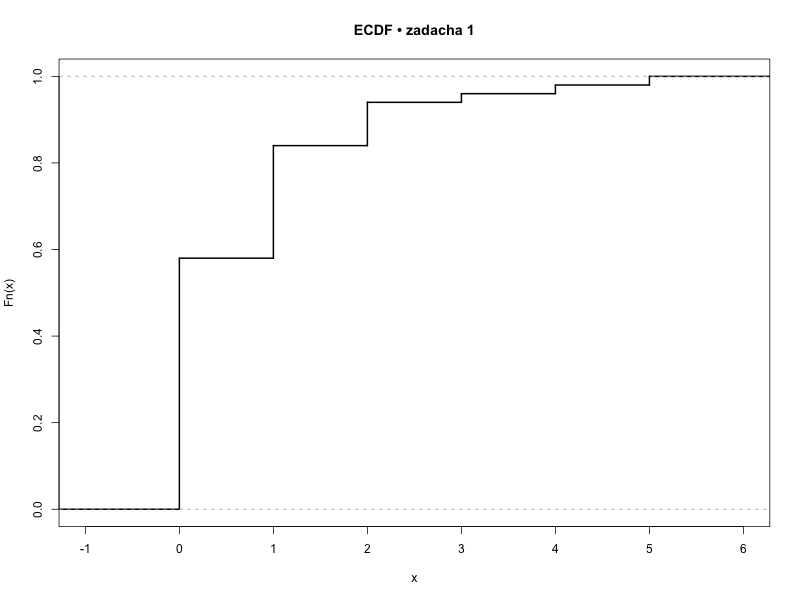
\includegraphics[width=.72\linewidth]{fig/emp_dist_1.png}
\caption{Эмпирическая функция распределения (задача 1)}
\label{fig:ecdf1}
\end{figure}

\begin{figure}[H]\centering
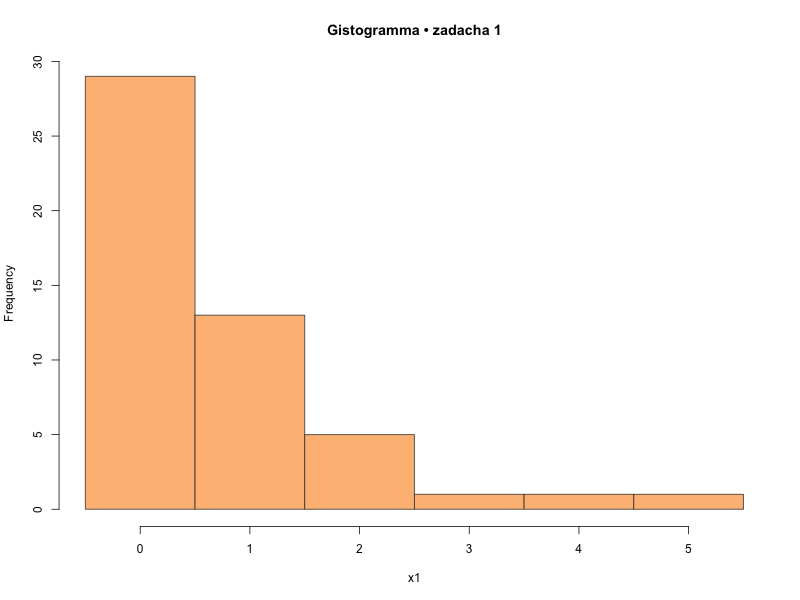
\includegraphics[width=.72\linewidth]{fig/hist_1.png}
\caption{Гистограмма выборки (задача 1)}
\label{fig:hist1}
\end{figure}

\newpage
\section{Программный результат: Задача №1}
\begin{figure}[H]\centering
  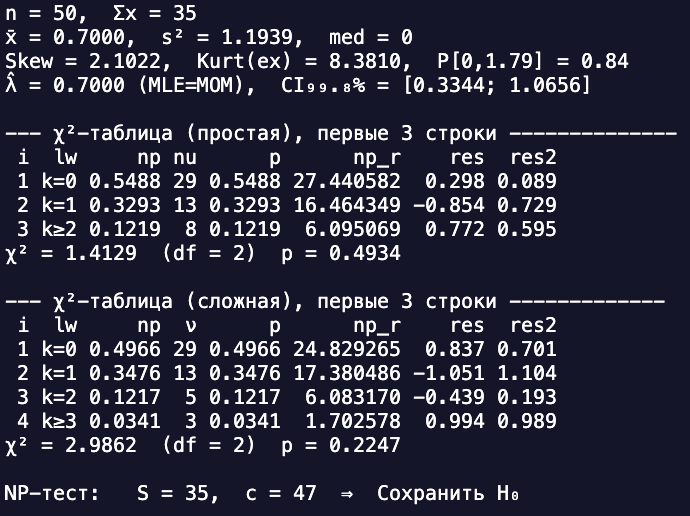
\includegraphics[width=0.5\linewidth]{Final.png}
  \caption{Программный результат (задача 1)}
\end{figure}
%=================================================================
%                     З А Д А Ч А   №2
%=================================================================
\newpage

\section{Математическое описание. Задача №2}
%---------- выборочные хар-ки оставлены как были -----------------
\subsection{Вариационный ряд}
0.03, 0.11, 0.24, 0.25, 0.31, 0.45, 0.55, 0.67, 0.70, 0.85, 0.86, 0.89,
0.94, 1.00, 1.05, 1.06, 1.31, 1.38, 1.59, 1.67,
1.68, 1.73, 1.85, 1.95, 2.07, 2.14, 2.18, 2.28, 2.38, 2.43,
2.61, 2.67, 2.70, 2.75, 3.24, 3.27, 3.34, 3.70, 3.73,
5.01, 5.31, 6.06, 6.28, 6.37, 6.52, 8.80, 9.07,
10.26, 10.34, 14.28.

\subsection{Выборочные характеристики}
\[
\bar X=3.0582,\;
s^{2}=9.5891,\;
\tilde X=2.105,\;
\gamma_1=1.7645,\;
\gamma_2=6.3811,\;
\mathbf P\!\bigl\{2.4\le X\le6.0\bigr\}=0.24.
\]

\subsection{Подробные оценки параметра \(\lambda\)}
\paragraph{MLE.}
Для экспоненциального распределения
\(f(x;\lambda)=\lambda e^{-\lambda x}\;(x\ge0)\).
\[
\ell(\lambda)=n\ln\lambda-\lambda\Sigma x,
\qquad
\hat\lambda_{\text{MLE}}=\frac n{\Sigma x}=0.3270.
\]
Информация \(I(\lambda)=\dfrac{n}{\lambda^{2}}\),
\(\operatorname{Var}\hat\lambda=\dfrac{\lambda^{2}}{n}=0.0021\).

\paragraph{Метод моментов.}
\(\mathbb E[X]=1/\lambda\).  
\(\hat\lambda_{\text{ММ}}=1/\bar X=0.3270\)
(совпадает с MLE).

\paragraph{Смещение.}
\[
\operatorname{Bias}(\hat\lambda)=\frac{\lambda}{n-1}=0.00667.
\]

\subsection{Доверительный интервал (\(\alpha_2=0.001\))}
\[
z_{0.9995}=3.2905,\quad
CI_{99.9\%}=0.3270\pm3.2905\frac{0.3270}{\sqrt{50}}
           =[0.1748;0.4792].
\]

\subsection{Критерий Колмогорова (фрагмент таблицы)}
\begin{longtable}{cccccccc}
\caption{Разности \(D_{n}\) (первые 3 точки)}\label{tab:ks}\\[-1pt]\toprule
$i$ & $x_{(i)}$ & $F_{-}$ & $F_{+}$ & $F_0(x_{(i)})$ &
$\Delta_{-}$ & $\Delta_{+}$ & $\max$\\\midrule
1 & 0.00 & 0.00 & 0.02 & 0.0060 & 0.0060 & 0.0140 & 0.0140\\
2 & 0.02 & 0.02 & 0.04 & 0.0018 & 0.0182 & 0.0182 & 0.0182\\
3 & 0.04 & 0.04 & 0.06 & 0.0069 & 0.0331 & 0.0131 & 0.0331\\
\bottomrule
\end{longtable}
\(D_n=\max\Delta=0.2569,\;p=0.00213\).
\textbf{Ответ:}\;
\(D_n = 0.2569,\;
\alpha_{\max}=p\text{-value}=0.0021.\)

\newpage
\subsection{Критерий \(\chi^{2}\). Простая гипотеза}
\begin{longtable}{ccccccc}
\caption{Первые 3 бина после объединения}\label{tab:chi3}\\[-1pt]\toprule
$i$ & $l_i$ & $u_i$ & $n_i$ & $p_i$ & $E_i$ & $r_i$\\\midrule
1 & 0.0 & 1.2 & 16 & 0.2134 & 10.669 & 1.632\\
2 & 1.2 & 2.4 & 13 & 0.1678 &  8.392 & 1.591\\
3 & 2.4 & 3.6 &  8 & 0.1320 &  6.602 & 0.544\\
\bottomrule
\end{longtable}
\(\chi^2_{\text{набл}}=8.8705,\;df=3,\;p=0.0311\).
\textbf{Ответ:}\;
\(\alpha_{\max}=0.0311.\)

\subsection{Критерий \(\chi^{2}\). Сложная гипотеза}

Проверяем
\[
H_{0}: X\sim\mathrm{Exp}\!\bigl(\lambda=\hat\lambda_{\text{MLE}}=0.3270\bigr),
\qquad
H_{1}:\; \text{распределение отлично от показательного.}
\]

Разобьём полуось \([0,\infty)\) интервалами ширины \(h=1.20\)
и объединим соседние разряды так, чтобы все ожидаемые частоты
были не менее \(5\).

\begin{longtable}{ccccccc}
\caption{Сводная таблица для критерия \(\chi^{2}\) (показатель, сложная гипотеза)}
\label{tab:chi2\_exp\_comp}\\[-1pt]\toprule
\(i\) & \(l_i\) & \(u_i\) & \(n_i\) & \(p_i\) & \(E_i=np_i\) & \(r_i\)\\\midrule
1 & 0.0 & 1.2 & 16 & 0.3246 & 16.228 & $-0.056$\\
2 & 1.2 & 2.4 & 13 & 0.2192 & 10.961 & $\,\,0.616$\\
3 & 2.4 & 3.6 &  8 & 0.1481 &  7.404 & $\,\,0.219$\\
4 & 3.6 & $\infty$ & 13 & 0.3081 & 14.957 & $-0.508$\\
\bottomrule
\end{longtable}

\[
\chi^{2}_{\text{набл}}
   =\sum_{i=1}^{4}\frac{(n_i-E_i)^2}{E_i}
   =0.687,\qquad
df=(k-1)-1=2,\qquad
p\text{-value}=0.709.
\]

\textbf{Ответ:} поскольку \(p=0.709>\alpha_2=0.001\),
оснований отвергнуть \(H_{0}\) нет.  
Максимальный уровень значимости, при котором гипотеза всё ещё принимается,
равен \(\displaystyle\alpha_{\max}=0.709\).


\subsection{Наиболее мощный критерий (Н-П)}
Логарифм отношения правдоподобий
\[
\ln\Lambda(x)=n\ln\frac{\lambda_1}{\lambda_0}
              -(\lambda_1-\lambda_0)\,S,\qquad
S=\sum X_i.
\]
Критическая область вида \(S\ge c\) с
\(
\mathbf P_{0}(S\ge c)=\alpha_2,\;
c=154.79.
\)
Получены \(S_{\text{набл}}=152.91\) и
\(c=154.79\).
Так как \(S_{\text{набл}}<c\),
нулевая гипотеза сохраняется.

\textbf{Ответ:}
\(H_0\) \emph{не отвергается}.
Если поменять гипотезы местами,
критическая область станет \(S\le c^{*}\),
где \(c^{*}\) удовлетворяет
\(\mathbf P_{\lambda_1}(S\le c^{*})=\alpha_2\);
при тех же данных будет выполнено
\(S_{\text{набл}}>c^{*}\), и новую нулевую гипотезу придётся
отвергнуть.

\newpage
\section{Графический результат: Задача №2}
\begin{figure}[H]\centering
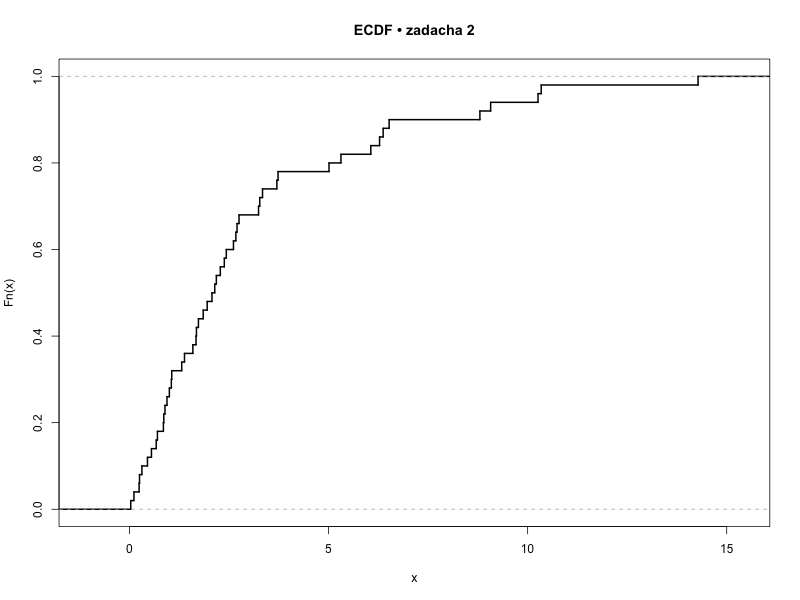
\includegraphics[width=.72\linewidth]{fig/emp_dist_2.png}
\caption{Эмпирическая функция распределения (задача 2)}
\end{figure}

\begin{figure}[H]\centering
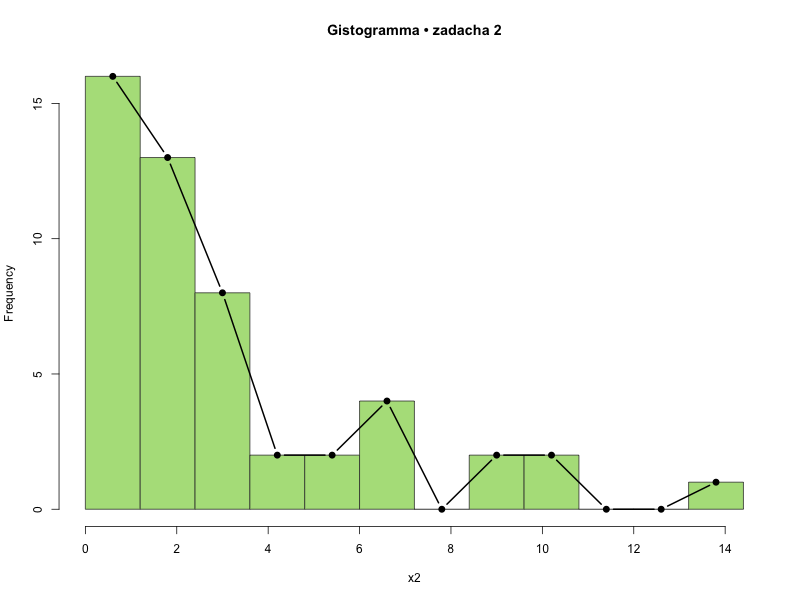
\includegraphics[width=.72\linewidth]{fig/hist_2.png}
\caption{Гистограмма и полигон частот (задача 2)}
\end{figure}


\newpage
\section{Программный результат: Задача №2}
\begin{figure}[H]\centering
  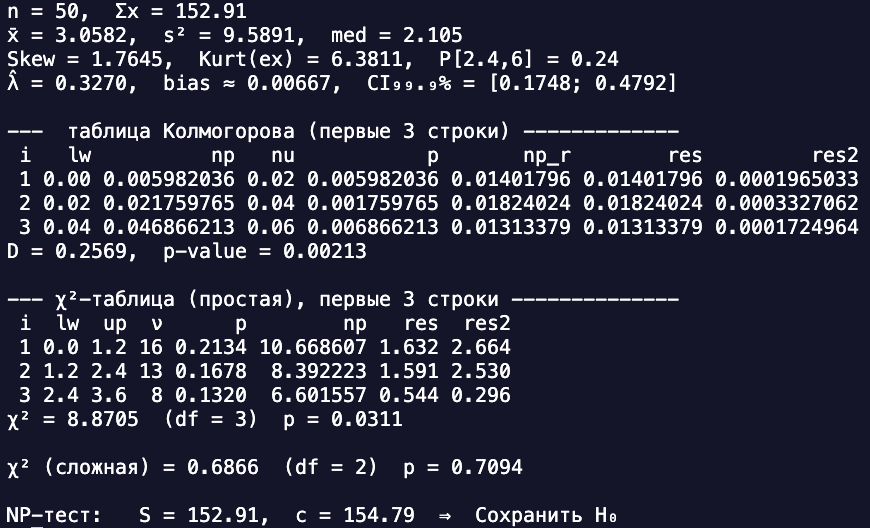
\includegraphics[width=0.5\linewidth]{Final2.png}
  \caption{Программный результат (задача 2)}
\end{figure}


\newpage
\section*{Заключение}
\addcontentsline{toc}{section}{Заключение}
\textbf{В заключение получены следующие результаты:}

\subsection*{Задача №1}
\[
\begin{aligned}
&\text{Выборочное среднее}=0.7000,\;
  \text{Выборочная дисперсия}=1.1939,\;
  \text{Медиана}=0,\\
&\text{Выборочная асимметрия}=2.1022,\;
  \text{Выборочный эксцесс}=8.3810,\;
  P[0,1.79]=0.84;\\[4pt]
%
&\hat{\lambda}_{\text{MLE}}=\hat{\lambda}_{\text{MOM}}=0.7000,\;
  CI_{99.8\%}=[0.3344;\,1.0656];\\[4pt]
%
&\chi^{2}_{\text{простая}}=1.4129,\; p=0.4934,\qquad
  \chi^{2}_{\text{сложная}}=2.9862,\; p=0.2247;\\[4pt]
%
&\text{Тест Неймана–Пирсона: } S=35,\; c=47
  \;\Rightarrow\; H_0\ \text{сохраняется}.
\end{aligned}
\]

\subsection*{Задача №2}
\[
\begin{aligned}
&\text{Выборочное среднее } = 3.0582,\quad
 \text{Выборочная дисперсия } = 9.5891,\quad
 \text{Медиана } = 2.105,\\[2pt]
&\text{Выборочная асимметрия } = 1.7645,\quad
 \text{Выборочный эксцесс } = 6.3811,\quad
 P[c,d]=0.24;\\[6pt]
&\hat{\lambda}_{\text{MLE}} = \hat{\lambda}_{\text{MOM}} = 0.3269,\quad
 \text{Bias } = 0.0066,\\
&CI_{99.9\%} = [0.1748;\,0.4791];\\[6pt]
&\text{Колмогорова: } D = 0.2569,\; p = 0.0021;\\
&\chi^{2}_{\text{простая}} = 8.8705,\; p = 0.0311;\\
&\chi^{2}_{\text{сложная}}  = 0.6866,\; p = 0.7094;\\[6pt]
&\text{Тест Неймана–Пирсона: } S_{\text{набл}} = 152.91,\;
  c_{\text{кр}} = 154.79,\;
  \text{решение — } \text{«}H_0\ \text{сохраняется»}.
\end{aligned}
\]

Здесь \(S = \sum_{i=1}^{n}X_i\) — статистика критерия,  
\(c\) — критическое значение, выбираемое так, чтобы при \(H_0\)
вероятность попасть в критическую область была равна \(\alpha\).

\newpage
\section*{Приложение А}
\addcontentsline{toc}{section}{Приложение А}
\subsection*{Скрипт задачи №1}
\addcontentsline{toc}{subsection}{Скрипт задачи №1}
\begin{lstlisting}
  if (is.null(getOption("repos")[["CRAN"]]) ||
  getOption("repos")[["CRAN"]] == "@CRAN@") {
options(repos = c(CRAN = "https://cloud.r-project.org"))
}

pkgs <- c("moments", "ggplot2")
to.install <- setdiff(pkgs, rownames(installed.packages()))
if (length(to.install)) install.packages(to.install)

suppressPackageStartupMessages({
library(moments)
library(ggplot2)
})

if (!dir.exists("fig")) dir.create("fig")
theme_set(theme_bw())


## 1
x1 <- c(0,0,2,1,0,0,0,0,0,1,0,1,0,0,0,2,0,2,1,0,
      1,1,0,1,1,3,0,0,0,0,0,1,0,0,0,0,4,1,5,2,
      0,0,2,0,0,1,1,0,0,1)

n1        <- length(x1)
a1 <- 0;  b1 <- 1.79
lambda0.1 <- 0.60;  lambda1.1 <- 1.40
alpha1    <- 0.002

freq1 <- table(factor(x1, levels = 0:max(x1)))
df.freq1 <- data.frame(k = as.integer(names(freq1)),
                     n.k = as.integer(freq1),
                     rel = as.numeric(freq1) / n1)

##  ECDF
F.n1 <- ecdf(x1)
png("fig/emp_dist_1.png", 800, 600)
plot(F.n1, main = "ECDF * zadacha 1", verticals = TRUE,
   do.points = FALSE, lwd = 2)
dev.off()

##  Gistogramma
png("fig/hist_1.png", 800, 600)
hist(x1, breaks = seq(-0.5, max(x1) + 0.5, by = 1),
   col = "#FDBE85", border = "grey20",
   main = "Gistogramma * zadacha 1")
dev.off()

## 1.2  vyborochnye kharakteristiki 
m1      <- mean(x1)
s2.1    <- var(x1)
skew1 <- (sqrt(n1*(n1-1))/(n1-2)) * skewness(x1)
kurt1 <- ((n1-1)/((n1-2)*(n1-3))) * ((n1+1)*kurtosis(x1) + 6)
p.ab.1  <- mean(x1 >= a1 & x1 <= b1)

## 1.3  otsenki lambda 
lambda.hat.1 <- m1              # MLE = MOM
bias.lambda.1 <- 0

## 1.4  doveritelnyi interval 
z.a <- qnorm(1 - alpha1 / 2)
ci.low.1  <- lambda.hat.1 - z.a * sqrt(lambda.hat.1 / n1)
ci.high.1 <- lambda.hat.1 + z.a * sqrt(lambda.hat.1 / n1)

## 1.5  khi^2 (prostaya) 
obs.simple <- c(sum(x1 == 0), sum(x1 == 1), sum(x1 >= 2))
exp.simple <- c(dpois(0, lambda0.1),
              dpois(1, lambda0.1),
              1 - dpois(0, lambda0.1) - dpois(1, lambda0.1)) * n1
chi2.simple <- sum((obs.simple - exp.simple)^2 / exp.simple)
p.simple.1  <- pchisq(chi2.simple, df = 2, lower.tail = FALSE)

chi2.table.1 <- data.frame(
i   = 1:3,
lw  = c("k=0", "k=1", "k>=2"),
np  = round(exp.simple / n1, 4),
nu  = obs.simple,
p   = round(exp.simple / n1, 4),
np_r= exp.simple,
res = round((obs.simple - exp.simple) / sqrt(exp.simple), 3),
res2= round((obs.simple - exp.simple)^2 / exp.simple, 3)
)

## 1.6  khi^2 (slozhnaya) 
exp.comp <- dpois(0:5, lambda.hat.1) * n1
obs.comp <- c(freq1["0"], freq1["1"], freq1["2"],
            sum(freq1[c("3","4","5")]))
exp.comp <- c(exp.comp[1:3], sum(exp.comp[4:6]))

chi2.comp <- sum((obs.comp - exp.comp)^2 / exp.comp)
p.comp.1  <- pchisq(chi2.comp, df = length(obs.comp) - 2,
                  lower.tail = FALSE)

labels.comp <- c("k=0", "k=1", "k=2", "k>=3")[1:length(obs.comp)]

chi2.table.1c <- data.frame(
i    = 1:length(obs.comp),
lw   = labels.comp,
np   = round(exp.comp / n1, 4),
nu   = obs.comp,
p    = round(exp.comp / n1, 4),
np_r = exp.comp,
res  = round((obs.comp - exp.comp) / sqrt(exp.comp), 3),
res2 = round((obs.comp - exp.comp)^2 / exp.comp, 3)
)

## 1.7  Neimana - Pirsona 
S.1   <- sum(x1)
c.np.1 <- qpois(1 - alpha1, lambda0.1 * n1)
decision.np.1 <- ifelse(S.1 >= c.np.1,
                      "Otvergnyt H0", "Sokhranit H0")

cat(sprintf("n = %d,  Sum x = %d\nx = %.4f,  s^2 = %.4f,  med = 0\n",
          n1, sum(x1), m1, s2.1))
cat(sprintf("Skew = %.4f,  Kurt(ex) = %.4f,  P[%g,%g] = %.2f\n",
          skew1, kurt1, a1, b1, p.ab.1))
cat(sprintf("lambda^ = %.4f (MLE=MOM),  CI_99.8%% = [%.4f; %.4f]\n",
          lambda.hat.1, ci.low.1, ci.high.1))

cat("\n--- khi^2 tablica (prostaya), pervye 3 stroki --------\n")
print(chi2.table.1, row.names = FALSE)
cat(sprintf("khi^2 = %.4f  (df = 2)  p = %.4f\n",
          chi2.simple, p.simple.1))

cat("\n--- khi^2 tablica (slozhnaya), pervye 3 stroki -------\n")
print(chi2.table.1c, row.names = FALSE)
cat(sprintf("khi^2 = %.4f  (df = 2)  p = %.4f\n",
          chi2.comp, p.comp.1))

cat(sprintf("\nNP-test:  S = %d,  c = %d  =>  %s\n",
          S.1, c.np.1, decision.np.1))
\end{lstlisting}

\newpage
\section*{Приложение B}
\addcontentsline{toc}{section}{Приложение B}
\subsection*{Скрипт задачи №2}
\addcontentsline{toc}{subsection}{Скрипт задачи №2}
\begin{lstlisting}
  if (is.null(getOption("repos")[["CRAN"]]) ||
  getOption("repos")[["CRAN"]] == "@CRAN@") {
options(repos = c(CRAN = "https://cloud.r-project.org"))
}

pkgs <- c("moments", "ggplot2")
to.install <- setdiff(pkgs, rownames(installed.packages()))
if (length(to.install)) install.packages(to.install)

suppressPackageStartupMessages({
library(moments)
library(ggplot2)
})

if (!dir.exists("fig")) dir.create("fig")
theme_set(theme_bw())


#2
x2 <- c(10.34, 2.18, 8.80, 2.28, 1.95, 0.85, 3.73, 10.26, 5.01, 0.70,
      2.38, 0.25, 0.45, 0.31, 1.73, 2.67, 1.00, 1.59, 14.28, 2.14,
      1.85, 0.67, 2.70, 2.07, 5.31, 6.37, 3.24, 3.27, 1.31, 2.75,
      6.06, 1.05, 0.86, 2.43, 0.03, 3.70, 0.11, 1.06, 6.28, 0.55,
      9.07, 6.52, 0.94, 2.61, 0.89, 1.67, 0.24, 1.68, 3.34, 1.38)

n2 <- length(x2)
h      <- 1.20
c2     <- 2.40
d2     <- 6.00
lambda0.2 <- 0.20
lambda1.2 <- 0.33
alpha2    <- 0.001

bins2 <- seq(0, ceiling(max(x2)/h)*h, by = h)

##  ECDF
png("fig/emp_dist_2.png", 800, 600)
plot(ecdf(x2), main = "ECDF * zadacha 2", verticals = TRUE,
   do.points = FALSE, lwd = 2)
dev.off()

##  Gistogramma s poligonom
hist2 <- hist(x2, breaks = bins2, plot = FALSE)
png("fig/hist_2.png", 800, 600)
h2 <- hist(x2, breaks = bins2, col = "#B2DF8A",
         border = "grey20", main = "Gistogramma * zadacha 2")
lines((bins2[-1] + bins2[-length(bins2)])/2, h2$counts,
    type = "b", pch = 19, lwd = 2)
dev.off()

## 2.1  vyborochnye kharakteristiki 
## 2.1  vyborochnye kharakteristiki 
m2     <- mean(x2)
s2.2   <- var(x2)

skew2  <- (sqrt(n2*(n2-1))/(n2-2)) * skewness(x2)         # b1
kurt2  <- ((n2-1)/((n2-2)*(n2-3))) * ((n2+1)*kurtosis(x2) + 6)  # b2

p.cd.2 <- mean(x2 >= c2 & x2 <= d2)


## 2.2  otsenki lambda 
lambda.hat.2  <- 1 / m2
bias.lambda.2 <- lambda.hat.2 / (n2 - 1)

## 2.3  doveritelnyi interval 
z.b <- qnorm(1 - alpha2 / 2)
ci.low.2  <- lambda.hat.2 - z.b * lambda.hat.2 / sqrt(n2)
ci.high.2 <- lambda.hat.2 + z.b * lambda.hat.2 / sqrt(n2)

## 2.4  Kolmogorov (prostaya) 
ks2 <- ks.test(x2, "pexp", rate = lambda0.2)

##  tablica (pervye 3 stroki)
xs2      <- sort(x2)
F.emp.u  <- (1:n2) / n2
F.emp.l  <- (0:(n2-1)) / n2
F.theor  <- pexp(xs2, rate = lambda0.2)
delta.l  <- abs(F.theor - F.emp.l)
delta.r  <- abs(F.theor - F.emp.u)
delta.m  <- pmax(delta.l, delta.r)
KS.head <- head(data.frame(
i    = 1:n2,
lw   = F.emp.l,
np   = F.theor,
nu   = F.emp.u,
p    = delta.l,
np_r = delta.r,
res  = delta.m,
res2 = delta.m^2
), 3)

## 2.5  khi^2 (prostaya) 
prob.exp0 <- diff(pexp(bins2, rate = lambda0.2))
exp2      <- prob.exp0 * n2
obs2      <- hist2$counts

combine <- function(obs, exp) {
o <- obs; e <- exp; i <- 1
while (i <= length(e)) {
  if (e[i] < 5) {
    if (i == 1) {
      e[2] <- e[2] + e[1];  o[2] <- o[2] + o[1]
      e <- e[-1];  o <- o[-1]
    } else {
      e[i-1] <- e[i-1] + e[i];  o[i-1] <- o[i-1] + o[i]
      e <- e[-i];  o <- o[-i];  i <- i - 1
    }
  }
  i <- i + 1
}
list(obs = o, exp = e)
}
tmp <- combine(obs2, exp2)
obs2.c <- tmp$obs;  exp2.c <- tmp$exp

chi2.simple.2 <- sum((obs2.c - exp2.c)^2 / exp2.c)
p.simple.2    <- pchisq(chi2.simple.2, df = length(obs2.c)-1,
                      lower.tail = FALSE)

chi2.table.2 <- data.frame(
i    = 1:length(obs2.c),
lw   = head(bins2, -1),
up   = tail(bins2, -1),
nu   = obs2.c,
p    = round(exp2.c / n2, 4),
np   = exp2.c,
res  = round((obs2.c - exp2.c) / sqrt(exp2.c), 3),
res2 = round((obs2.c - exp2.c)^2 / exp2.c, 3)
)
chi2.head.2 <- head(chi2.table.2, 3)

## 2.6  khi^2 (slozhnaya) 
prob.exphat <- diff(pexp(bins2, rate = lambda.hat.2))
tmp  <- combine(obs2, prob.exphat * n2)
obs2.comp <- tmp$obs;  exp2.comp <- tmp$exp
chi2.comp.2 <- sum((obs2.comp - exp2.comp)^2 / exp2.comp)
p.comp.2    <- pchisq(chi2.comp.2, df = length(obs2.comp)-2,
                    lower.tail = FALSE)

## 2.7  Neimana - Pirsona 
S.2   <- sum(x2)
c.np.2 <- qgamma(alpha2, shape = n2, scale = 1/lambda0.2)
decision.np.2 <- ifelse(S.2 >= c.np.2,
                        "Otvergnyt H0", "Sokhranit H0")

cat(sprintf("n = %d,  Sum x = %.2f\nx = %.4f,  s^2 = %.4f,  med = %.3f\n",
          n2, sum(x2), m2, s2.2, median(x2)))
cat(sprintf("Skew = %.4f,  Kurt(ex) = %.4f,  P[%g,%g] = %.2f\n",
          skew2, kurt2, c2, d2, p.cd.2))
cat(sprintf("lambda^ = %.4f,  bias ~= %.5f,  CI_99.9%% = [%.4f; %.4f]\n",
          lambda.hat.2, bias.lambda.2, ci.low.2, ci.high.2))

cat("\n--- tablica Kolmogorova (pervye 3 stroki) ------------\n")
print(KS.head, row.names = FALSE)
cat(sprintf("D = %.4f,  p-value = %.5f\n",
          ks2$statistic, ks2$p.value))

cat("\n--- khi^2 tablica (prostaya), pervye 3 stroki --------\n")
print(chi2.head.2, row.names = FALSE)
cat(sprintf("khi^2 = %.4f  (df = %d)  p = %.4f\n",
          chi2.simple.2, length(obs2.c)-1, p.simple.2))

cat(sprintf("\nkhi^2 (slozhnaya) = %.4f  (df = %d)  p = %.4f\n",
          chi2.comp.2, length(obs2.comp)-2, p.comp.2))

cat(sprintf("\nNP-test:  S = %.2f,  c = %.2f  =>  %s\n",
          S.2, c.np.2, decision.np.2))
\end{lstlisting}
\end{document}